\section{实验内容\cite{pcl2002,pku2002physicalchem}}

\subsection{仪器与药品}

环己烷 $(A R)$,无水乙醇 $(A R)$,丙酮 $(A R)$。

恒沸点仪,阿贝折射仪,温度测定及加热控制装置,导线,$30 \mathrm{~mL}$ 滴瓶 (公用),1、2、5 和 20$ \mathrm{~mL}$ 移液管各两只,滴管。

\subsection{实验步骤与条件}

\begin{figure}[H]
   \centering
   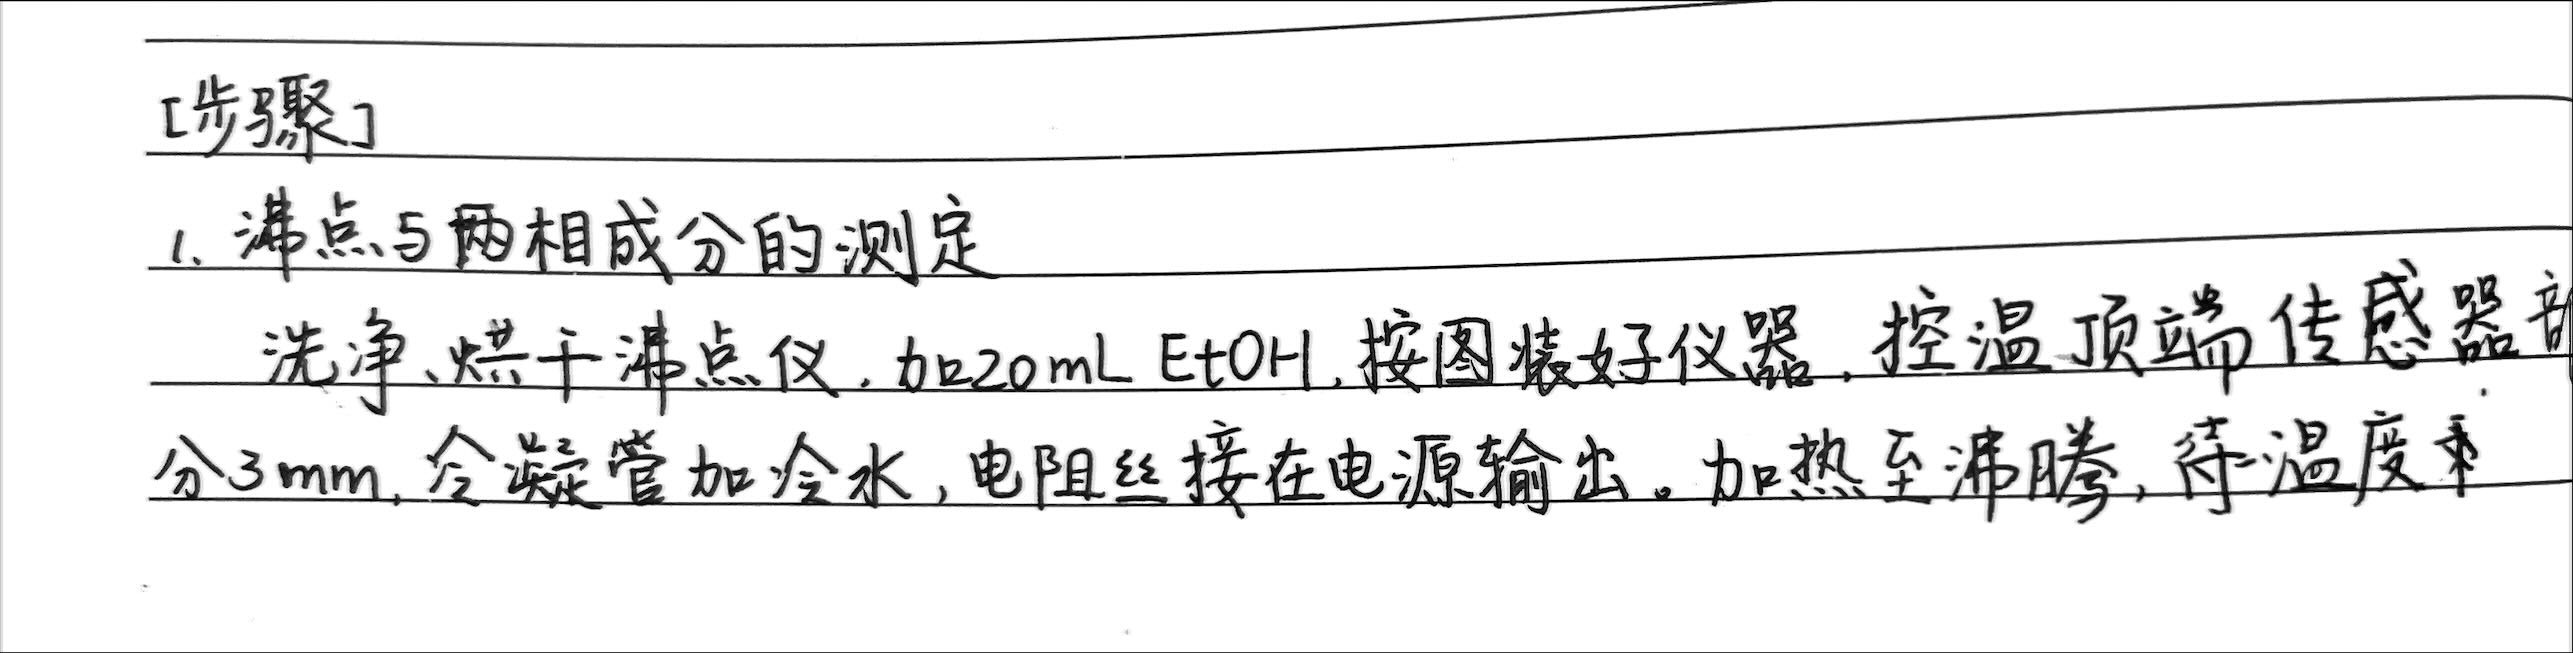
\includegraphics[width=.78\textwidth]{figures/0-2-1.jpg}
   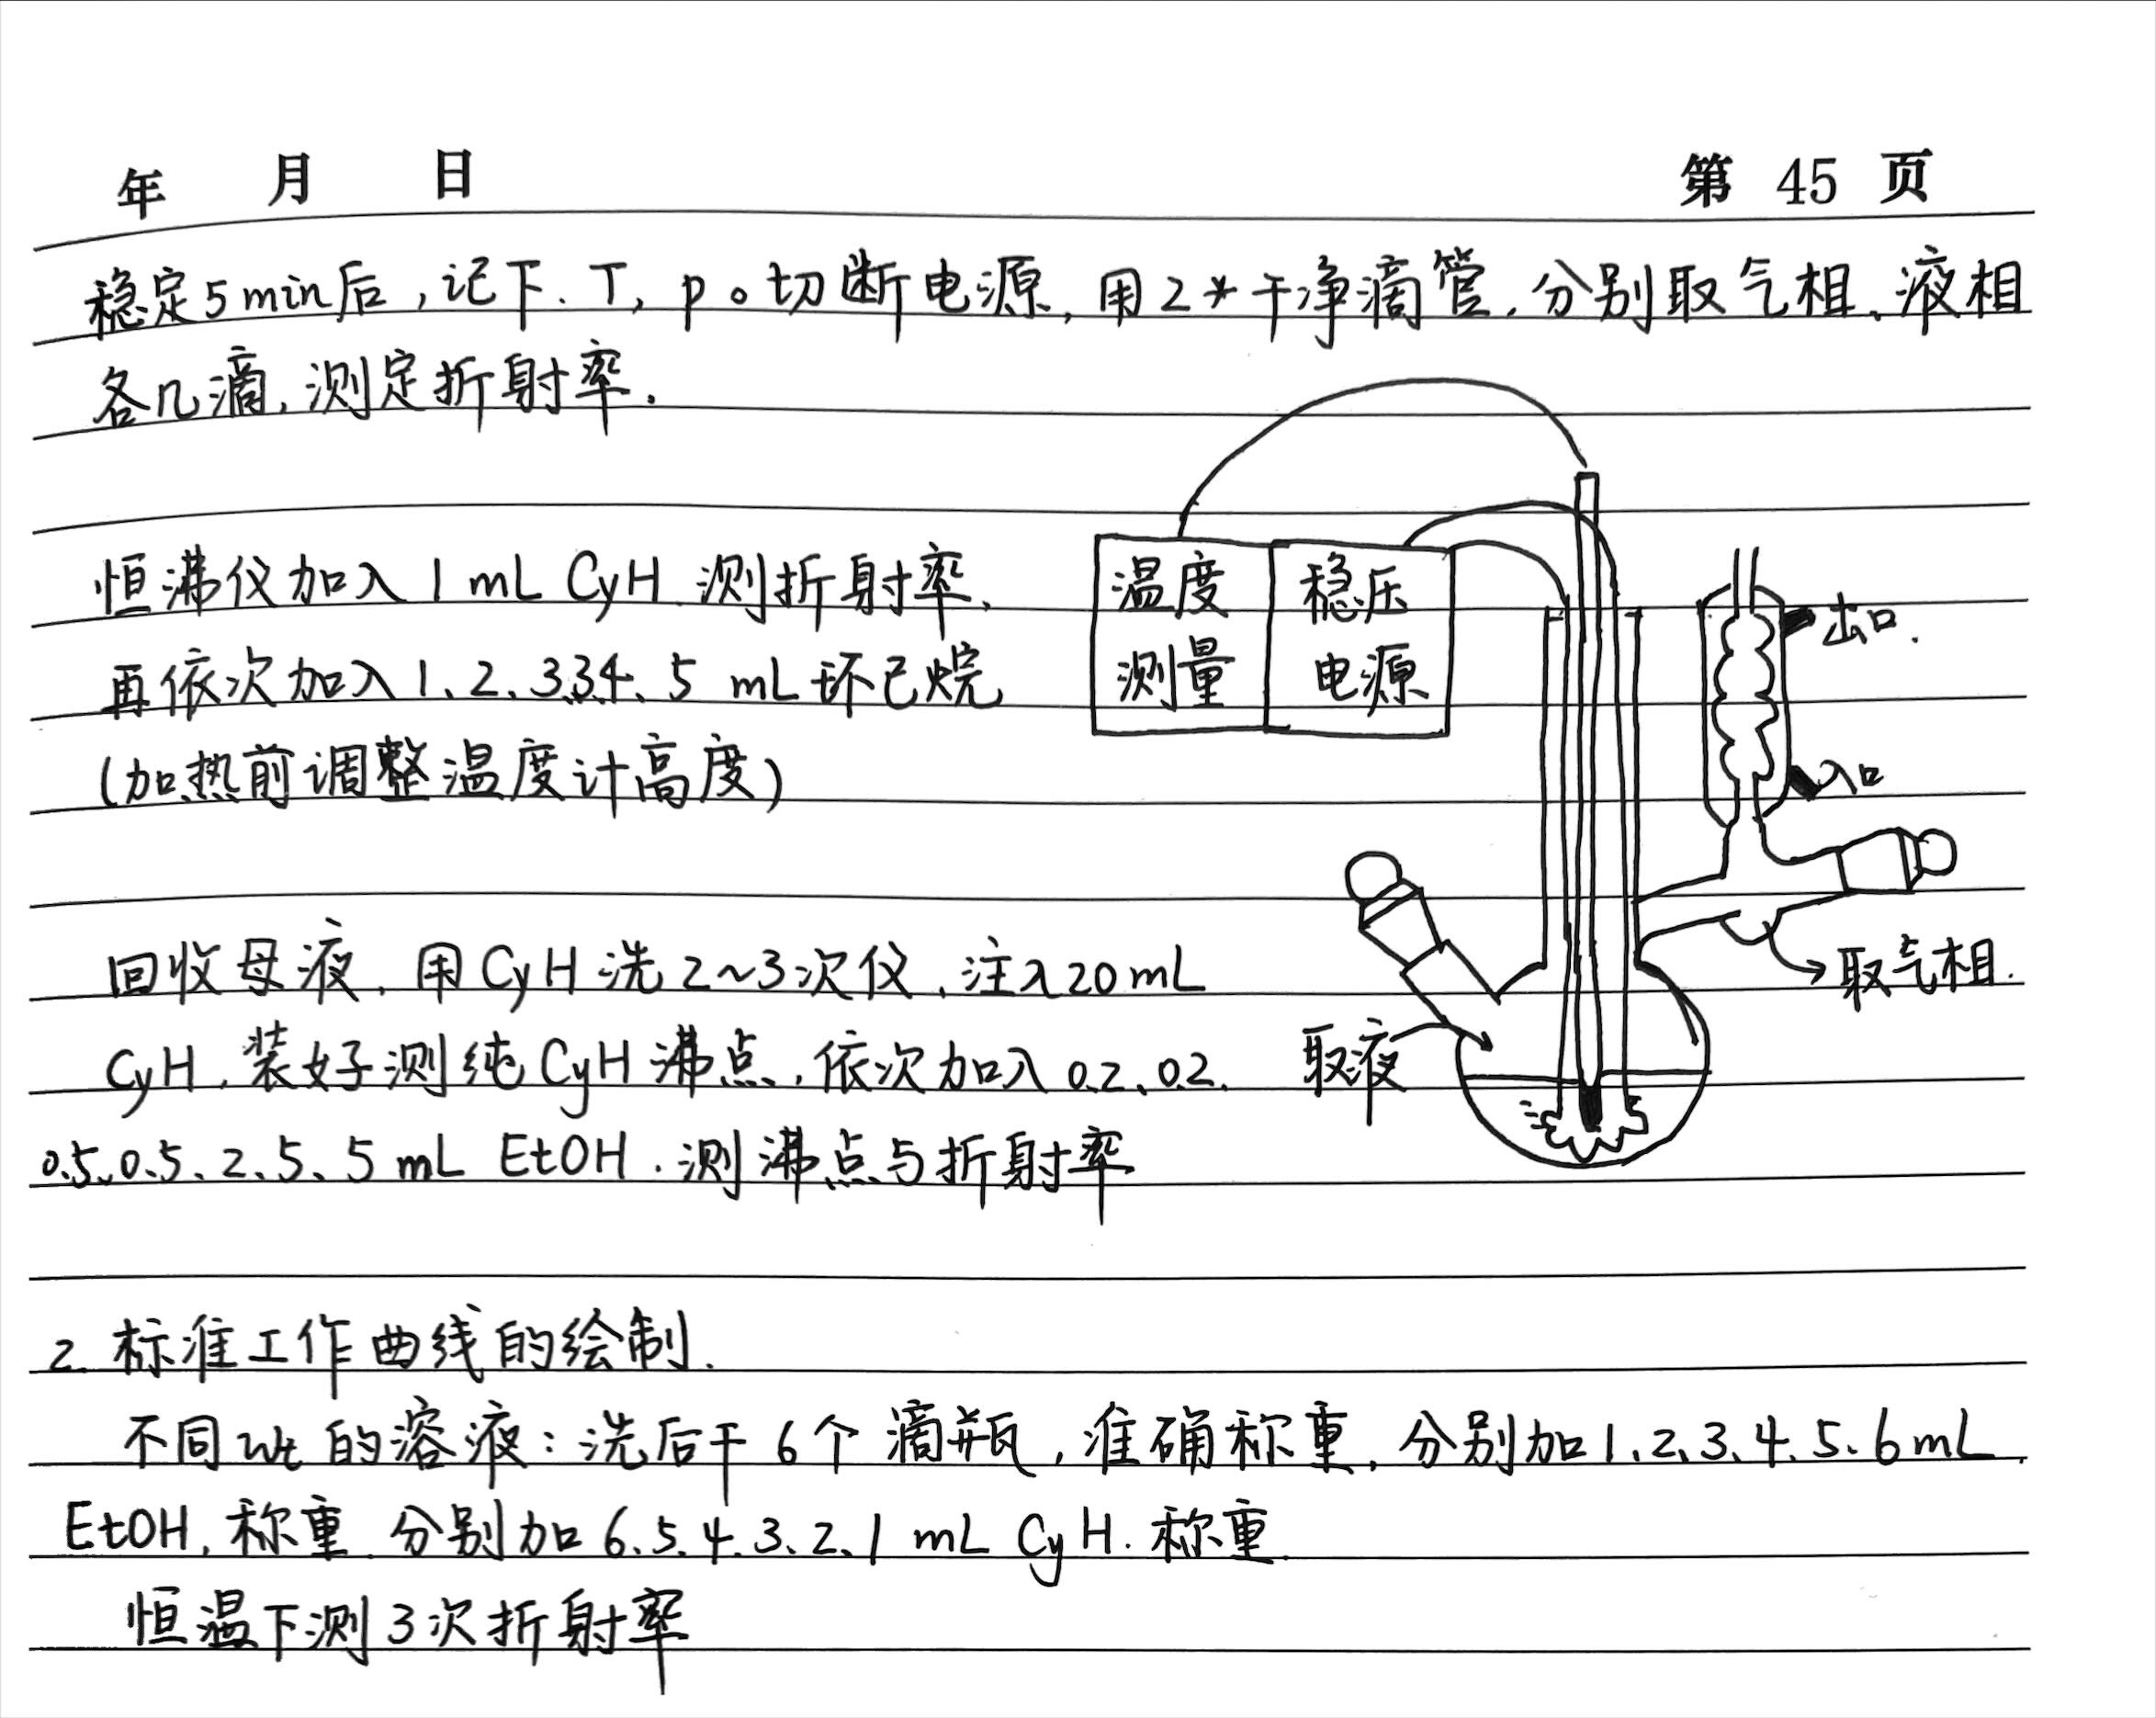
\includegraphics[width=.78\textwidth]{figures/0-2-2.jpg}
   \bicaption{实验步骤与条件}{Schematic Diagram of Experimental Apparatus}

\end{figure}

\subsection{沸点和两相成分的测定}

蒸馏瓶加入 $20 \mathrm{~mL}$ 乙醇,装好仪器,温度计的热电偶底端一半浸入液体内、一半在液体上的空气中,冷凝管内通入冷水。将电阻丝接在输出电压 $12.6 \mathrm{~V}$ 的变压器上,使温度升高并沸腾。待温度稳定后数分钟,记下温度及大气压。切断电源,用两支干净的滴管,分别取出支管处的气相冷凝液和蒸馏瓶中的液体几滴,立即使用阿贝折射仪测定其折射率。

蒸馏瓶中加入 $1 \mathrm{~mL}$ 环己烷,按前述方法测定平衡沸点 $t_b$ 及气相折射率 $n^g$ 、液相折射率 $n^l$ 。再依次加入 $1.00 \mathrm{~mL} $、$ 2.00 \mathrm{~mL} $、$ 3.00 \mathrm{~mL} $、$ 3.00 \mathrm{~mL} $、$ 4.00 \mathrm{~mL} $、$ 5.00 \mathrm{~mL}$ 环已烷,记录液体组成,进行同样的实验。

上述实验结束后,回收母液,再用少量环已烷洗 $3 \sim 4$ 次蒸馏瓶,注入 $20.00 \mathrm{~mL}$ 环己烷,再装好仪器。先测定纯环己烷的沸点,然后依次加入 $0.20 \mathrm{~mL} $、$ 0.20 \mathrm{~mL} $、$ 0.50 \mathrm{~mL}$ $、$ $0.50 \mathrm{~mL} $、$ 2.00 \mathrm{~mL} $、$ 2.00 \mathrm{~mL} $、$ 5.00 \mathrm{~mL} $、$ 5.00 \mathrm{~mL}$ 乙醇,分别测定平衡沸点 $t_b$ 及气相折射率 $n^g$ 、液相折射率 $n^l$ 。

\subsection{标准工作曲线绘制}


取 8 个干净的小滴瓶,冷却后准确称量其质量 $m_0$ 。用带刻度的移液管分别加入 $1.00 \mathrm{~mL}$ $、$ $2.00 \mathrm{~mL} $、$ 3.00 \mathrm{~mL} $、$ 4.00 \mathrm{~mL} $、$ 5.00 \mathrm{~mL} $、$ 6.00 \mathrm{~mL}$、$ 7.00 \mathrm{~mL}$、$ 8.00 \mathrm{~mL}$ 乙醇,分别称量其质量 $m_1$,再依次分别加入 $ 8.00 \mathrm{~mL}$、$ 7.00 \mathrm{~mL}$、$6.00 \mathrm{~mL} $、$ 5.00 \mathrm{~mL} $、$ 4.00 \mathrm{~mL} $、$ 3.00 \mathrm{~mL} $、$ 2.00 \mathrm{~mL} $、$ 1.00 \mathrm{~mL}$ 环已烷,再分别称量其质量 $m_2$,旋紧盖子后摇匀。
在恒温 $t=30.1\si{\celsius}$ 下分别测定这些样品的折射率 $n$ 。

